\documentclass{article}
\usepackage[utf8]{inputenc}
\usepackage{graphicx} 
\usepackage{import}
\usepackage{imakeidx} 
\usepackage{amsmath}
\usepackage{amssymb}
\usepackage{pdfpages}
\usepackage{array}
\usepackage{float} 
\usepackage{multicol}
\usepackage{listings} 
\usepackage{url}
\usepackage{natbib}
\usepackage{csquotes}
\usepackage{caption}
\usepackage{xcolor}   
\usepackage{geometry}

\geometry{top=25mm, bottom=25mm, left=20mm, right=20mm}
\setlength{\parindent}{0pt}
\renewcommand\contentsname{Index}

\begin{document}

\import{./}{cover.tex}
\tableofcontents

% Abstract
\section*{Abstract}

This project presents the design, development, and implementation of the movement module for a mobile social robot intended to manage access to microwaves in a university environment. The goal was to create a compact, autonomous platform capable of omnidirectional navigation, basic obstacle detection, and integration with future functional modules.

The mechanical structure consists of cut wooden platforms joined by vertical columns, housing all electronic and mechanical components. Movement is enabled by three DC motors with omnidirectional wheels, arranged in a triangular configuration, and controlled by motor drivers. A microcontroller governs the system, handling PWM motor control and ultrasonic sensor input, powered by a regulated LiPo battery setup.

The development process focused on early testing of individual components through a modular setup, followed by full system integration on the final chassis. The resulting prototype delivers a robust and adaptable movement platform, capable of supporting higher-level behaviors and other modules. It provides a solid foundation for building a functional and socially engaging service robot.


% Phase 1: Discover
\section{Phase 1: Discover}

During the discovery phase, the team organized its structure, established roles for management, conducted research and developed initial proposals for the module.

\subsection{Team Organization}

Our team is composed of five students:
\begin{itemize}
    \item \textbf{Ermelinda Giulivo}
    \item \textbf{Rafael Monllor Ballesteros}
    \item \textbf{Daniel Mauricio Ruiz Suarez}
    \item \textbf{Jurij Diego Scandola}
    \item \textbf{Abdul Moiz}
\end{itemize}

The team leader and \textbf{Backbone member} is Jurij Diego Scandola.

Our responsibilities and roles are:
\begin{itemize}
    \item \textbf{Rapporteur}: Rafael Monllor Ballesteros
    \item \textbf{Schedule manager}: Jurij Diego Scandola
    \item \textbf{Art director}: Daniel Mauricio Ruiz Suarez
    \item \textbf{Tech manager}: Ermelinda Giulivo
    \item \textbf{Designer}: Abdul Moiz
\end{itemize}

\subsection{Project Management}

Our team plans to solve the tasks according to the following GANTT:

\begin{figure}[H]
    \centering
    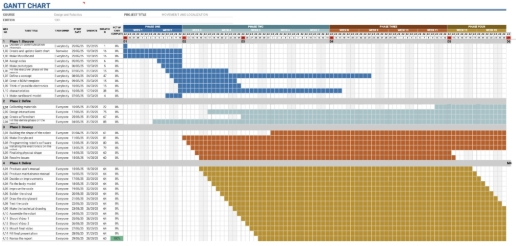
\includegraphics[width=0.85\linewidth]{../ReportMovementModule/images/Aspose.Words.728084da-df58-4b9d-a372-f65cffbdb23d.001.jpeg}
    \caption{Project GANTT Chart}
\end{figure}

\subsection{Research}

The research phase is a critical foundation for the development of the movement and localization module of the indoor robot. At this stage, the primary objective is to explore and analyse existing technologies, methodologies and systems that enable precise navigation and positioning within indoor environments. Unlike outdoor settings, indoor environments present unique challenges such as signal attenuation, dynamic obstacles and limited access to GPS, making robust and reliable localization and movement a complex task.

\subsection{Omnidirectional Movement Approach}

For the movement and localization module of the indoor robot, an \textbf{omnidirectional movement} approach has been selected. This strategy enables the robot to move seamlessly in any direction without the need to rotate its chassis first. Typically implemented using omni-wheels or mecanum wheels, omnidirectional systems are particularly advantageous in constrained and dynamic indoor environments. However, this choice also comes with certain trade-offs.

\begin{itemize}
    \item \textbf{Enhanced Manoeuvrability:} Omnidirectional movement allows for instant lateral, diagonal or rotational motion. This is highly beneficial in tight spaces or crowded indoor environments where flexibility is critical.
    \item \textbf{Simplified Path Planning:} Since the robot can move in any direction at any time, path planning algorithms can be more straightforward compared to traditional differential drive systems, reducing complexity in navigation.
    \item \textbf{Improved Positioning Accuracy:} Fine adjustments to the robot's position and orientation are easier, which is crucial for tasks that demand high precision, such as docking, object manipulation or alignment tasks.
    \item \textbf{Smooth Obstacle Avoidance:} The ability to sidestep obstacles without complex turning manoeuvres leads to smoother and often faster responses in dynamic environments.
\end{itemize}

\textbf{Limitations:}
\begin{itemize}
    \item \textbf{Mechanical Complexity:} Omni-wheels and their assemblies are more mechanically intricate than standard wheels, potentially leading to higher manufacturing costs and increased maintenance needs.
    \item \textbf{Lower Traction and Load Capacity:} Due to the design of omni-wheels (which often rely on small rollers), they typically offer less traction and may struggle on uneven surfaces, affecting stability and limiting the robot's carrying capacity.
    \item \textbf{Energy Efficiency:} Omnidirectional systems can be less energy-efficient, especially during complex movement patterns, leading to increased power consumption.
    \item \textbf{Control Challenges:} Maintaining accurate and stable movement requires more sophisticated control algorithms. Wheel slip and small errors in motion can accumulate, potentially affecting localization accuracy if not properly managed.
\end{itemize}

\subsection{Defining the Number of Wheels: Three-Wheel vs. Four-Wheel Omnidirectional Configurations}

After selecting an omnidirectional movement strategy, the next major design challenge was to determine the optimal number of wheels for the robot. Specifically, we needed to choose between a \textbf{three-wheel} and a \textbf{four-wheel} omnidirectional configuration. This decision plays a critical role in the robot's stability, manoeuvrability, mechanical complexity and overall performance.

\textbf{Three-Wheel Omnidirectional Configuration}
\begin{itemize}
    \item \textbf{Advantages:} Simplicity, compact design, sufficient mobility.
    \item \textbf{Disadvantages:} Reduced stability, weight distribution challenges, limited redundancy.
\end{itemize}

\textbf{Four-Wheel Omnidirectional Configuration}
\begin{itemize}
    \item \textbf{Advantages:} Greater stability, improved traction, increased redundancy.
    \item \textbf{Disadvantages:} Higher mechanical complexity, larger footprint.
\end{itemize}

\subsection{Defining the Robot’s Shape: Square, Circular, Polygonal or Triangular Designs}

Following the decisions on movement type and wheel configuration, another crucial design consideration was the \textbf{shape} of the robot's base. The geometry of the robot directly affects not only its aesthetic but also its \textbf{manoeuvrability}, \textbf{stability}, \textbf{sensor placement} and \textbf{ability to navigate tight indoor spaces}. The primary shapes considered were \textbf{square}, \textbf{circular}, \textbf{polygonal} and \textbf{triangular} forms, each offering distinct advantages and challenges.

\begin{itemize}
    \item \textbf{Square:} Symmetry, ease of design, but corners can get caught and less smooth navigation.
    \item \textbf{Circular:} Excellent manoeuvrability, ideal for dynamic environments, but less space-efficient and more complex to construct.
    \item \textbf{Polygonal:} Balance between round and angular, unique structural advantages, but more complex to design and assemble.
    \item \textbf{Triangular:} Compact, simple three-wheel integration, but limited stability and challenging payload distribution.
\end{itemize}

\subsection{Group Cardboard Prototype Proposals}

When tasked with creating a cardboard prototype of the module, the group presented four different design proposals with detailed analysis of their advantages and disadvantages.

\subsubsection{Omnidirectional robot with four wheels positioned at the vertices of a square}

\textbf{Proposed by:} Ermelinda Giulivo

\begin{figure}[H]
    \centering
    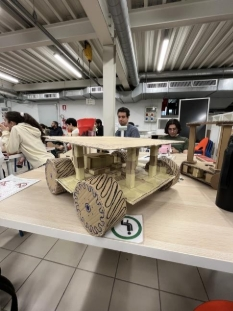
\includegraphics[width=0.5\linewidth]{../ReportMovementModule/images/Aspose.Words.728084da-df58-4b9d-a372-f65cffbdb23d.002.jpeg}
    \caption{Square-based Omnidirectional Robot}
\end{figure}

\begin{table}[H]
\centering
\begin{tabular}{|p{0.45\textwidth}|p{0.45\textwidth}|}
\hline
\multicolumn{2}{|c|}{\textbf{Omnidirectional robot with four wheels positioned at the vertices of a square}} \\
\hline
\textbf{Pros} & \textbf{Cons} \\
\hline
\textbf{Excellent Stability:} The square layout provides a wide and balanced support base, enhancing stability, especially when carrying payloads or navigating uneven indoor floors. & \textbf{Larger Turning Radius Compared to Circular Robots:} Although it can strafe and rotate, the square footprint is bulkier when fitting into very tight or irregularly shaped spaces. \\
\hline
\textbf{Full Omnidirectional Mobility:} With wheels positioned symmetrically, the robot can move smoothly in any direction — forward, backward, sideways or diagonally — without needing to rotate first. & \textbf{Wheel Synchronization Complexity:} Precise control of all four wheels is essential. Small discrepancies in motor performance can cause drift or errors in movement if not properly calibrated. \\
\hline
\textbf{Simple Mechanical Symmetry:} The square design makes mechanical construction easier and ensures even distribution of forces, reducing stress on the frame. & \textbf{Higher Energy Consumption:} Coordinated omnidirectional movement (especially diagonal motion) can be less energy-efficient compared to simpler drive systems. \\
\hline
\textbf{Good for Sensor Placement:} The square chassis offers clear and logical positions for sensors, allowing for easy 360-degree coverage with minimal blind spots. & \textbf{Cost and Mechanical Complexity:} Four omni-wheels and corresponding motors, encoders and controllers increase system cost and complexity compared to simpler two-wheel or three-wheel robots. \\
\hline
\textbf{Predictable and Balanced Control:} Because of the symmetry, the control algorithms (e.g., for velocity distribution across wheels) can be simpler and more consistent. & \textbf{Vulnerability to Wheel Slippage:} Omni-wheels rely on small rollers, which can slip on smooth or dusty indoor surfaces, potentially affecting localization accuracy. \\
\hline
\end{tabular}
\end{table}

\subsubsection{Triangular-shaped, three-wheel omnidirectional robot}

\textbf{Proposed by:} Rafael Monllor Ballesteros

\begin{figure}[H]
    \centering
    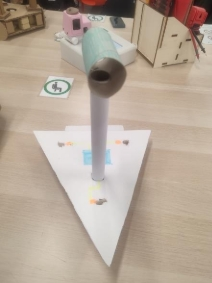
\includegraphics[width=0.5\linewidth]{../ReportMovementModule/images/Aspose.Words.728084da-df58-4b9d-a372-f65cffbdb23d.003.jpeg}
    \caption{Triangular-shaped Omnidirectional Robot}
\end{figure}

\begin{table}[H]
\centering
\begin{tabular}{|p{0.45\textwidth}|p{0.45\textwidth}|}
\hline
\multicolumn{2}{|c|}{\textbf{Triangular-shaped, three-wheel omnidirectional robot}} \\
\hline
\textbf{Pros} & \textbf{Cons} \\
\hline
\textbf{Compact Design:} Three wheels in a triangular configuration create an optimally compact base while still maintaining stability. & \textbf{Lower Weight Distribution Stability:} Compared to four-wheel designs, triangular bases provide less stability for tall or top-heavy constructions. \\
\hline
\textbf{Less Mechanical Complexity:} One fewer motor and wheel compared to four-wheel designs means fewer components to maintain, calibrate, and potentially fail. & \textbf{More Complex Control Algorithms:} Achieving precise omnidirectional movement with three wheels can require more sophisticated software than four-wheel configurations. \\
\hline
\textbf{Lower Power Consumption:} Operating three motors instead of four reduces total energy usage, potentially extending battery life. & \textbf{Potential Payload Limitations:} The triangular base may support less weight or require more careful weight distribution than square configurations. \\
\hline
\textbf{Efficient for Small Robots:} Ideal for light-duty applications where high payload capacity is not necessary. & \textbf{Less Redundancy:} If one motor or wheel fails, the robot's ability to move properly is much more compromised than with four-wheel designs. \\
\hline
\end{tabular}
\end{table}

\subsubsection{Polygonal-shaped omnidirectional robot with four wheels arranged in a cross configuration}

\textbf{Proposed by:} Daniel Mauricio Ruiz Suarez

\begin{figure}[H]
    \centering
    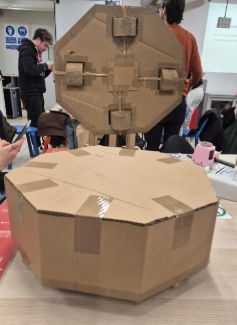
\includegraphics[width=0.5\linewidth]{../ReportMovementModule/images/Aspose.Words.728084da-df58-4b9d-a372-f65cffbdb23d.004.jpeg}
    \caption{Polygonal-shaped Robot with Cross Wheel Configuration}
\end{figure}

\begin{table}[H]
\centering
\begin{tabular}{|p{0.45\textwidth}|p{0.45\textwidth}|}
\hline
\multicolumn{2}{|c|}{\textbf{Polygonal-shaped omnidirectional robot with four wheels arranged in a cross configuration}} \\
\hline
\textbf{Pros} & \textbf{Cons} \\
\hline
\textbf{Optimized Use of Space:} The polygonal chassis (such as hexagonal or octagonal) better fits the cross pattern while allowing more efficient internal layout of components compared to a purely circular design. & \textbf{Design Complexity:} More complicated to design and assemble compared to pure circular or square robots. \\
\hline
\textbf{Simplified Path Planning:} Because the wheels are symmetrically arranged, control algorithms for movement and localization become more predictable and manageable. & \textbf{Potential for Increased Size:} Depending on the polygon shape and wheel placement, the overall footprint of the robot could become larger than necessary for tight indoor environments. \\
\hline
\textbf{Better Obstacle Navigation:} The extended wheel positions can help in negotiating tight spaces or approaching obstacles at different angles more smoothly. & \textbf{Higher Control Precision Needed:} Maintaining synchronized wheel movement across a cross configuration demands precise motor control to avoid unwanted drift or vibration, especially at higher speeds. \\
\hline
\textbf{Load Distribution Sensitivity:} Uneven weight distribution can negatively affect movement performance, as each wheel may bear different loads during turns or fast translations. & \\
\hline
\end{tabular}
\end{table}

\subsubsection{Circular-shaped, three-wheel omnidirectional robot}

\textbf{Proposed by:} Jurij Diego Scandola

\begin{figure}[H]
    \centering
    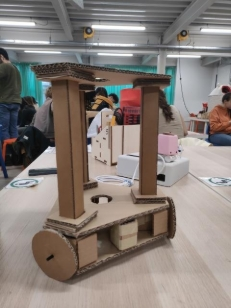
\includegraphics[width=0.5\linewidth]{../ReportMovementModule/images/Aspose.Words.728084da-df58-4b9d-a372-f65cffbdb23d.005.jpeg}
    \caption{Circular-shaped Omnidirectional Robot}
\end{figure}

\begin{table}[H]
\centering
\begin{tabular}{|p{0.45\textwidth}|p{0.45\textwidth}|}
\hline
\multicolumn{2}{|c|}{\textbf{Circular-shaped, three-wheel omnidirectional robot}} \\
\hline
\textbf{Pros} & \textbf{Cons} \\
\hline
\textbf{Excellent Manoeuvrability:} The circular design eliminates corners, allowing smooth and uninterrupted movement and rotation in any direction — ideal for navigating tight, cluttered indoor environments. & \textbf{Reduced Structural Simplicity:} Building a strong, circular chassis (especially with flat materials like cardboard or sheet metal) can be mechanically more complex compared to square or polygonal shapes. \\
\hline
\textbf{Compact and Symmetrical:} The circular form naturally distributes mass and components around the centre, enhancing balance and improving dynamic stability during motion. & \textbf{Lower Load Capacity:} Three-wheel setups naturally provide less stability and support for heavy loads compared to four-wheel configurations and the circular frame can limit internal mounting options for large or heavy components. \\
\hline
\textbf{Efficient for Omnidirectional Control:} The 120° placement of the three wheels around the circle simplifies omnidirectional movement algorithms and ensures consistent movement performance. & \textbf{Challenging Internal Layout:} Fitting rectangular or square components (like batteries, boards, and sensors) inside a circular space can be inefficient and may lead to wasted internal volume. \\
\hline
\textbf{Minimal Risk of Snagging:} Without edges or corners, the robot can more easily avoid getting caught on obstacles, furniture, or tight doorways. & \textbf{Sensitivity to Weight Imbalance:} Proper balancing is critical; even slight asymmetry in weight distribution can significantly impact the robot's movement precision and stability. \\
\hline
\textbf{Aesthetically Appealing:} The circular shape often results in a cleaner, more modern appearance, which can be a factor in user-facing or commercial applications. & \textbf{Less Redundancy:} With only three wheels, if one wheel or motor fails, the robot's mobility is seriously compromised compared to a four-wheel design. \\
\hline
\end{tabular}
\end{table}

\subsection{Selected Approach}

After evaluating all prototype designs, the group decided on a modified polygonal approach that incorporated a \textbf{dodecagonal (12-sided) base} with \textbf{three omnidirectional wheels} arranged in a triangular configuration. This combined the stability advantages of a wide base with the mechanical simplicity of a three-wheel system.

\begin{figure}[H]
    \centering
    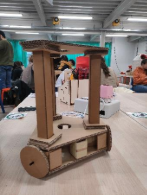
\includegraphics[width=0.5\linewidth]{../ReportMovementModule/images/Aspose.Words.728084da-df58-4b9d-a372-f65cffbdb23d.006.png}
    \caption{Final Cardboard Prototype}
\end{figure}

This approach offered several advantages:
\begin{itemize}
    \item The polygonal shape approximated a circle for smooth navigation while being easier to fabricate from flat materials
    \item Using three wheels reduced complexity and power consumption compared to four-wheel designs
    \item The wide base provided good stability without excessive weight
    \item The design allowed for sensor placement around the perimeter with minimal blind spots
    \item The balanced triangular wheel arrangement facilitated simple yet effective omnidirectional control
\end{itemize}

These early tests helped us set a clearer direction for both technical and conceptual development, bridging the gap between idea and implementation.

\subsection{Selecting the Sensing Technology: LiDAR, Ultrasonic, Camera and Other Options}

An essential step in developing the movement and localization module is selecting the \textbf{appropriate sensing technology}. The choice of sensors directly impacts the robot’s ability to perceive its environment, perform accurate localization, avoid obstacles and navigate efficiently indoors. Different types of sensors offer different strengths and weaknesses depending on the operating environment, required precision, cost and computational complexity.

\begin{itemize}
    \item \textbf{LiDAR:} High precision mapping, good range, strong performance in low light, but high cost and computational load.
    \item \textbf{Ultrasonic Sensors:} Low cost, simplicity, lightweight, but limited precision and susceptible to noise.
    \item \textbf{Cameras (RGB or Depth):} Rich environmental information, cost-effective, versatile, but lighting dependence and complex processing.
    \item \textbf{Other Options:}
    \begin{itemize}
        \item \textbf{IMU:} Provides orientation and movement data, but sensitive to drift.
        \item \textbf{Infrared Sensors:} Good for simple proximity detection, but limited in range and precision.
        \item \textbf{Magnetic Sensors:} Useful for specific localization systems using magnetic markers, but not practical for general indoor navigation.
    \end{itemize}
\end{itemize}

\subsection{Group Cardboard Prototype Proposals}

When tasked with creating a cardboard prototype of the module, the group presented four different design proposals.

\subsubsection{Omnidirectional robot with four wheels positioned at the vertices of a square}
\textit{Proposed by: Ermelinda Giulivo}

\begin{figure}[H]
    \centering
    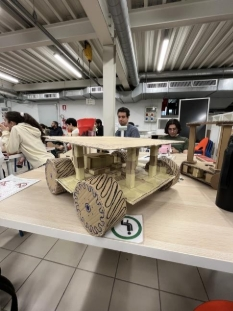
\includegraphics[width=0.6\linewidth]{../ReportMovementModule/images/Aspose.Words.728084da-df58-4b9d-a372-f65cffbdb23d.002.jpeg}
    \caption{Four-wheel square configuration prototype}
\end{figure}

\subsubsection{Triangular-shaped, three-wheel omnidirectional robot}
\textit{Proposed by: Rafael Monllor Ballesteros}

\begin{figure}[H]
    \centering
    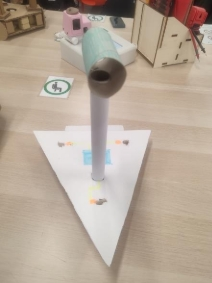
\includegraphics[width=0.6\linewidth]{../ReportMovementModule/images/Aspose.Words.728084da-df58-4b9d-a372-f65cffbdb23d.003.jpeg}
    \caption{Triangular three-wheel configuration prototype}
\end{figure}

\subsubsection{Polygonal-shaped omnidirectional robot with four wheels arranged in a cross configuration}
\textit{Proposed by: Daniel Mauricio Ruiz Suarez}

\begin{figure}[H]
    \centering
    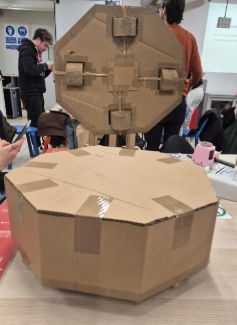
\includegraphics[width=0.6\linewidth]{../ReportMovementModule/images/Aspose.Words.728084da-df58-4b9d-a372-f65cffbdb23d.004.jpeg}
    \caption{Polygonal cross-wheel configuration prototype}
\end{figure}

\subsubsection{Circular-shaped, three-wheel omnidirectional robot}
\textit{Proposed by: Jurij Diego Scandola}

\begin{figure}[H]
    \centering
    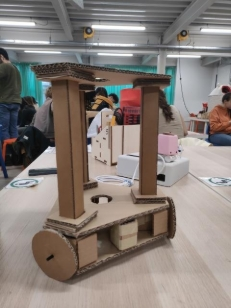
\includegraphics[width=0.6\linewidth]{../ReportMovementModule/images/Aspose.Words.728084da-df58-4b9d-a372-f65cffbdb23d.005.jpeg}
    \caption{Circular three-wheel configuration prototype}
\end{figure}


% Phase 2: Define
\section{Phase 2: Define}

After conducting broad research on existing social robots, user needs, and contextual use within shared spaces like university buildings, we moved on to define more specific goals for our own robot. Our challenge was to design a friendly, autonomous assistant capable of organizing turns for a shared microwave, while maintaining a mobile and socially engaging presence.

In this phase, we started shaping our concept through rough prototypes to test:

\begin{itemize}
    \item Basic \textbf{movement mechanisms} using omnidirectional wheels.
    \item \textbf{Aesthetic identity}, considering a space between two separated bases for hiding the electronics.
    \item Key \textbf{functionalities}, for getting a proper movement of the robot.
\end{itemize}

The cardboard prototype that best adjusted to these ideas can be seen in the following picture.

\begin{figure}[H]
    \centering
    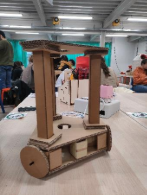
\includegraphics[width=0.6\linewidth]{../ReportMovementModule/images/Aspose.Words.728084da-df58-4b9d-a372-f65cffbdb23d.006.png}
    \caption{Cardboard prototype}
\end{figure}

These early tests helped us set a clearer direction for both technical and conceptual development, bridging the gap between idea and implementation.

\subsection{Strategy}

Our strategy during this phase focused on transforming abstract ideas into concrete design and implementation plans for the movement module of the robot. We followed a structured approach to ensure consistency across form, function, and technology.

\begin{enumerate}
    \item \textbf{Defining functionalities}
    
    We began by clearly outlining the movement module's responsibilities: patrolling the space, pausing at predefined locations to allow human interaction, and navigating autonomously to the charging station when battery levels are low. These core behaviors served as a foundation for every subsequent design decision.

    \item \textbf{Considering the physical form}
    
    We aimed to create a friendly and humorous appearance aligned with the social nature of the robot. The form of a cooking pot was chosen for its simplicity, roundness, and instantly recognizable shape, which also fits thematically with the microwave queue scenario.

    \item \textbf{Designing the 3D model of the movement module}
    
    Using 3D modeling tools, we created a rough prototype of the movement module's structure. This model focused on the chassis and physical arrangement of elements such as omnidirectional wheels, base support, and electronic housing. It helped us evaluate size constraints, stability, and potential mounting points for components.

    \item \textbf{Selecting electronic components}
    
    We identified the necessary electronic components, including three omnidirectional wheels, motor drivers, a microcontroller (ESP32), sensors for obstacle detection and battery monitoring, and components for the ticket dispensing system. We also defined the logical wiring and signal flow between them.

    \item \textbf{Beginning software development}
    
    In parallel, we started building the logic behind the movement module in code. This included route planning, obstacle avoidance, pausing logic, and low battery detection routines.
\end{enumerate}

\subsection{Functionalities}

The movement module was designed to enable the robot to perform three key behaviors: patrol autonomously through a mapped environment, stop periodically to allow interaction with users, and navigate to a charging station when the battery level is low. These main functionalities can be seen in the following flow chart:

\begin{figure}[H]
    \centering
    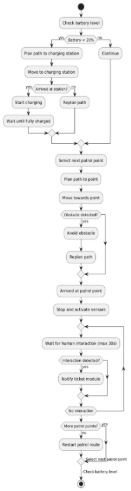
\includegraphics[width=0.8\linewidth]{../ReportMovementModule/images/Aspose.Words.728084da-df58-4b9d-a372-f65cffbdb23d.007.jpeg}
    \caption{Movement Module Flowchart}
\end{figure}

\subsection{Electronics}

The design of the electronics during the development phase was guided by the functional needs of the movement module. At this stage, we focused on defining a system that would enable \textbf{precise motor control}, allow for \textbf{basic sensing capabilities}, and remain \textbf{modular and scalable} for future upgrades.

Given that the robot needed to move holonomically using \textbf{three omnidirectional wheels}, it was essential to control \textbf{three independent DC motors} with precision. This required a microcontroller with multiple PWM-capable digital outputs and a structure that allowed us to drive each motor bidirectionally. We selected the \textbf{ATmega328P} microcontroller, due to its compatibility with the Arduino platform, which offered a familiar programming environment, low-level control, and access to a wide library of tested code.

To drive the motors, we needed reliable motor drivers that could handle the current demand and support direction and speed control. We opted for \textbf{DRV8871 single-channel H-bridge drivers}, one for each motor. These components provided sufficient current capacity, protection features, and a straightforward interface with the \textbf{ATmega328P}, using two digital pins per driver.

In addition to movement, the robot needed a basic level of \textbf{obstacle detection} to eventually navigate or stop when required. For this, we planned the integration of \textbf{ultrasonic sensors (HC-SR04)} around the perimeter. These sensors are simple, affordable, and widely used in robotics, but they require careful timing to avoid interference between readings. The ATmega328P offered enough GPIOs to connect up to six sensors, with logic implemented to trigger them sequentially.

All components would be powered by a \textbf{LiPo battery}, but since the system needed a stable 5V supply for both logic-level components and sensor operation, we included a \textbf{step-down voltage regulator (LM2596)} in the plan. This ensured consistent voltage despite the battery's natural variation underload.

From a wiring and assembly perspective, we anticipated the need to route motor cables and sensor wires efficiently between the top and bottom of the chassis. This led us to consider a vertical layout, with the \textbf{motor drivers placed near the motors} (on the bottom of the base), and the \textbf{microcontroller and logic-level components mounted on top}, minimizing wire length and simplifying troubleshooting.

In short, the electronics defined in this phase were selected not just for their individual performance, but for their ability to \textbf{integrate seamlessly} within a compact, layered robot structure, and support \textbf{clear, testable behaviors} during the next implementation stages.

\subsection{Coding}

The code developed so far focuses on the core functionalities of the movement module: patrolling the environment, stopping periodically for interaction, and returning to a charging station when battery levels are low. The code is being developed in C++, using the Arduino framework, since it offers:

\begin{itemize}
    \item High compatibility with our chosen microcontroller (ATmega328P).
    \item Access to well-documented libraries for motor control, timers, and sensors.
    \item A simple structure that facilitates rapid prototyping and debugging.
\end{itemize}

The microcontroller is programmed directly via the Arduino IDE, allowing us to flash and test code iterations easily. The robot can switch between various behaviors such as:

\begin{itemize}
    \item Patrolling predefined points.
    \item Stopping and waiting for user interaction.
    \item Navigating to the charging station when the battery is low.
\end{itemize}

In this phase, we focused on:

\begin{itemize}
    \item Defining key states and transitions.
    \item Mapping out which pins control each motor and sensor.
    \item Testing the motors and sensors.
\end{itemize}

The code used for the testing of the HC-SR04 ultrasonic sensors, and the motors can be seen in the Appendix.

\subsection{Structure}

The physical structure of the movement module was designed to be simple, stable, and compatible with the circular "cooking pot" appearance of the final robot. Its geometry allows for efficient assembly and proper distribution of electronic components, motors, and wheels. The chassis consists of two main dodecagonal plates:

\begin{itemize}
    \item A \textbf{lower base plate} that holds the motors, wheels, the battery, and electronics.
    \item An \textbf{upper plate} connected by four vertical rods, providing structural support and space for mounting future upper modules (such as the ticket dispenser).
\end{itemize}

Between the two plates, there's ample vertical space to safely house the internal wiring and maintain separation between moving and static parts. The structural elements were dimensioned using CAD software and detailed in the following technical drawings.

\begin{figure}[H]
    \centering
    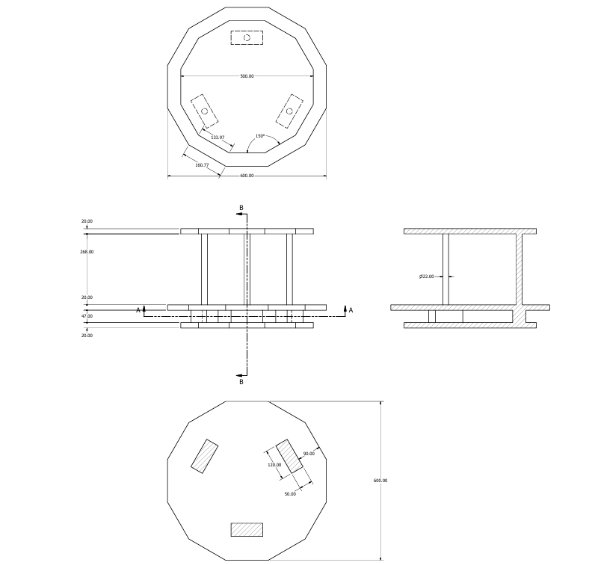
\includegraphics[width=0.7\linewidth]{../ReportMovementModule/images/Aspose.Words.728084da-df58-4b9d-a372-f65cffbdb23d.008.jpeg}
    \caption{Structure Technical Drawings}
\end{figure}

The structure is primarily symmetrical, promoting balance and helping the robot move stably in any direction. This design prioritizes modularity, allowing individual parts to be adjusted, replaced, or expanded without affecting the rest of the system.

\subsection{Shape}

The shape of the robot was designed to convey friendliness, uniqueness, and a sense of purpose within its social environment. Taking inspiration from kitchen elements, the robot adopts a stylized form reminiscent of a cooking pot, reinforcing its role as a ticket dispenser for a microwave queue.

The overall geometry is conical, with a wide dodecagonal base that houses the movement module and narrows as it rises, creating a silhouette that is both functional and expressive. The lower section (in red) is where the wheels and internal electronics are stored. The transparency of the conical section allows for visual access to internal components and lighting, adding both a technological and playful aesthetic.

At the top of the robot, the head is formed by a metallic-looking circular cap with a symmetrical design, integrating visual sensors, lights, or interface points. A pair of stylized "ears" or "handles" give it a characterful appearance, reinforcing its role as a social entity that invites interaction. The shape also leaves space at the front for a clearly visible ticket dispensing area.

\begin{figure}[H]
    \centering
    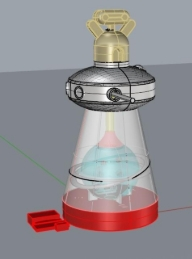
\includegraphics[width=0.6\linewidth]{../ReportMovementModule/images/Aspose.Words.728084da-df58-4b9d-a372-f65cffbdb23d.009.jpeg}
    \caption{Robot Shape Design}
\end{figure}

\subsection{Concept}

The concept behind our robot is to create a social and functional assistant that organizes the use of a shared microwave in a university environment.

By dispensing turn tickets and patrolling the space autonomously, the robot aims to bring order to an otherwise chaotic or informal process, while adding an element of humor and engagement through its unique design.

Inspired by everyday kitchen objects, its cooking pot-like appearance makes the robot immediately relatable and non-intimidating, encouraging students to approach it easily. Its ability to move, pause, and react transforms a mundane waiting experience into a playful and organized interaction, promoting better coexistence in shared spaces.

The combination of functionality and personality defines the essence of this project:

\textbf{a robot that not only helps manage tasks but also becomes a memorable part of its environment.}


% Phase 3: Develop
\section{Phase 3: Develop}

In this phase we describe the development process, departing from the first prototype to the final improvements regarding strategy, electronics, coding, structure, and shape.

% Additional Phase 3 sections will be added here

% Phase 4: Deliver
% Final Robot description
% Strategy
% Shape
% Mechanics
% Electronics
% Informatics

% Conclusion

% Appendix

% Minutes of the Meetings

% Bibliography

\end{document}
